
% This LaTeX was auto-generated from MATLAB code.
% To make changes, update the MATLAB code and republish this document.

\documentclass{article}
\usepackage{graphicx}
\usepackage{color}

\sloppy
\definecolor{lightgray}{gray}{0.5}
\setlength{\parindent}{0pt}

\begin{document}

    
    
\section*{Math 315: Lab 3}

\begin{par}
The following lab uses MATLAB functions to compute norms and condition numbers to analyze the difference in error between GEPP and using the inverse of a matrix. These errors are then used to check the validity of the bounds derived in the problem set.
\end{par} \vspace{1em}

\subsection*{Contents}

\begin{itemize}
\setlength{\itemsep}{-1ex}
   \item Procedure 1
   \item Procedure 2
\end{itemize}


\subsection*{Procedure 1}

\begin{par}
In the first procedure, I will randomly generate 10 random matrices A with a random vector b and solve Ax=b. Using MatLab's svd function, I will create two random orthogonal matrices U and V. I will then discard the singular values and generate them using a log scale. Then, I will compute the matrix A = U * S * V'. I will then be able to calculate the accurate inverse of A, with only double precision round-off errors. Using this accurate inverse, I will be able to calculate the accurate solution x, which can then be used to compare the GEPP and inverse matrix solutions.
\end{par} \vspace{1em}
\begin{verbatim}
n = 256;
sigma_1 = 10^4;
sigma_n = 10^-4;

rel_backward_err_inv = zeros(10, 1);
rel_forward_err_inv  = zeros(10, 1);
rel_backward_err_gepp = zeros(10, 1);
rel_forward_err_gepp  = zeros(10, 1);

saved_A = zeros(256,256,10);

for i = 1:10
    % Generate random matrix A, where the accurate inverse of A can be
    % accurately computed
    [U, ~, V] = svd(randn(n));
    svalues = logspace(log10(sigma_1), log10(sigma_n), n);
    S = diag(svalues);
    invS = diag(svalues.^-1);
    A = U * S * V';
    AccurateInv = V * invS * U';
    Z = inv(A);

    % Save A for future use
    saved_A(:,:,i) = A;

    % Generate random vector b and calculate forward/backward error for
    % solution x via inverse of A and GEPP
    b = randn(n, 1);
    x = V * (invS * (U' * b));
    xz = Z * b;
    xg = linsolve(A, b);
    rel_backward_err_inv(i) = norm(A * xz - b) / (norm(A) * norm(xz) + norm(b));
    rel_forward_err_inv(i)  = norm(xz - x) / norm(x);
    rel_backward_err_gepp(i) = norm(A * xg - b) / (norm(A) * norm(xg) + norm(b));
    rel_forward_err_gepp(i)  = norm(xg - x) / norm(x);
end

random_A_errs_inv = table(rel_backward_err_inv, rel_forward_err_inv, ...
    'VariableNames', {'Backward_Err_via_Z', 'Forward_Err_via_Z'});
disp(['Table of Relative Backward and Forward Error of Solutions of 10 Random ' ...
    'Matrices A and vectors b via Inverse Z']);
disp(random_A_errs_inv);

random_A_errs_gepp = table( rel_backward_err_gepp, rel_forward_err_gepp, ...
    'VariableNames', {'Backward_Err_via_GEPP', 'Forward_Err_via_GEPP'});
disp(['Table of Relative Backward and Forward Error of Solutions of 10 Random ' ...
    'Matrices A and vectors b via GEPP']);
disp(random_A_errs_gepp);

random_A_errs_comparison = table(abs(rel_backward_err_inv) ./ abs(rel_backward_err_gepp), ...
    abs(rel_forward_err_inv) ./ abs(rel_forward_err_gepp), ...
    'VariableNames', {'Ratio of Backward Err from Inverse to GEPP', ['Ratio ' ...
    'Forward Err from Inverse to GEPP']});
disp(['Table of Ratios of Relative Backward and Forward Error from Inverse Z ' ...
    'to GEPP for Solutions of 10 Random Matrices A and vectors b. (Ratio = |err ' ...
    'via inverse Z| - |err via GEPP|)']);
disp(random_A_errs_comparison);
\end{verbatim}

        \color{lightgray} \begin{verbatim}Table of Relative Backward and Forward Error of Solutions of 10 Random Matrices A and vectors b via Inverse Z
     Backward_Err_via_Z      Forward_Err_via_Z  
    ____________________    ____________________
    1.08841017918066e-15    1.98931543048129e-09
    7.93008182162173e-16    1.77102460563433e-09
    8.23732911729905e-16    2.49427619317505e-09
     1.1883281597749e-15    2.01644437929567e-09
    6.93278404597045e-16    3.25886965023931e-09
    1.13648624172882e-15    1.72136433518803e-09
    9.49780575701435e-16     2.1368640113379e-09
    6.44051290097859e-16    2.05521422380552e-09
    8.83612758336429e-16    1.67566141745073e-09
    8.88267171021903e-16    2.79690643756968e-09
Table of Relative Backward and Forward Error of Solutions of 10 Random Matrices A and vectors b via GEPP
    Backward_Err_via_GEPP    Forward_Err_via_GEPP
    _____________________    ____________________
    1.16972318298601e-16     1.98931455560678e-09
    1.97543096119835e-16     1.77102501440063e-09
    1.77694754824616e-16     2.49427709324709e-09
    1.68523270866152e-16     2.01644414735626e-09
    1.37404789831705e-16     3.25886901661003e-09
    1.39421533095454e-16     1.72136229331434e-09
    1.28775517240587e-16     2.13686336700363e-09
    1.46904626756133e-16     2.05521439846668e-09
    1.73853461365958e-16     1.67566151524465e-09
    1.31177983238241e-16     2.79690495069418e-09
Table of Ratios of Relative Backward and Forward Error from Inverse Z to GEPP for Solutions of 10 Random Matrices A and vectors b. (Ratio = |err via inverse Z| - |err via GEPP|)
    Ratio of Backward Err from Inverse to GEPP    Ratio Forward Err from Inverse to GEPP
    __________________________________________    ______________________________________
                 9.30485259257857                            1.00000043978691           
                 4.01435533682793                           0.999999769192249           
                  4.6356625019288                           0.999999639145128           
                 7.05141879615379                            1.00000011502397           
                 5.04551846734151                            1.00000019443226           
                 8.15143985650148                            1.00000118619636           
                 7.37547474903162                            1.00000030153274           
                  4.3841457163021                           0.999999915015601           
                  5.0825146154349                            0.99999994163862           
                 6.77146537165968                             1.0000005316146           
\end{verbatim} \color{black}
    \begin{par}
In the tables above, it's evident that solving systems using GEPP generally has lower relative backward error than using the inverse Z as all the values in the table of ratios between relative backward error of inverse Z to that of GEPP are greater than 1. However, there isn't a massive difference as the ratio isn't in the orders of magnitude of 10. Therefore, using the inverse Z to solve a linear system will be generally as accurate as GEPP, having around 1 decimal place of accuracy less than GEPP. Looking at the errors themself, it seems like they are all around the magnitude of epsilon meaning that the relative backward error seems to be bounded by epsilon time some small constant. This suggests that the O(machine epsilon) bound for backwards error of GEPP is accurate.
\end{par} \vspace{1em}
\begin{par}
To test if the bound is accurate for backwards error of inverse Z, I will calculate the bound using the last matrix calculated and compare with the largest relative backward error for inverse Z. As shown below the bound for relative backward error for inverse Z is also quite accurate.
\end{par} \vspace{1em}
\begin{verbatim}
norm_A_inv = norm(AccurateInv);
norm_xz = norm(xz);
norm_b = norm(b);

fprintf('Bound = O((||A^-1|| * ||b|| * 2*10^-16) / (||xz||) ~= %e\n', ...
    norm_A_inv .* norm_b .* eps() ./ norm_xz);
fprintf('Largest actual error ~= %e\n', max(abs(rel_backward_err_inv)));
\end{verbatim}

        \color{lightgray} \begin{verbatim}Bound = O((||A^-1|| * ||b|| * 2*10^-16) / (||xz||) ~= 1.637062e-15
Largest actual error ~= 1.188328e-15
\end{verbatim} \color{black}
    \begin{par}
For relative forward error, the ratio is almost nearly one for every entry. This follows from equations (1.5) and (1.6) that show the bounds of relative forward error for solutions via GEPP and inverse Z are equal if Z is a sufficiently accurate inverse.
\end{par} \vspace{1em}
\begin{par}
I will use the calculated condition numbers below for the different matrices A to check if the bounds described in (1.5) and (1.6) are reasonable. Since they are all approximately 10\^{}8 as shown below and the error bounds are approximately 10\^{}8 * 2 * 10\^{}-16 = 2 * 10\^{}-8, which is just greater than the calculated relative errors. Hence, the bounds described in equations (1.5) and (1.6) are quite accurate.
\end{par} \vspace{1em}
\begin{verbatim}
for i=1:10
    c = cond(saved_A(:,:,i));
    fprintf('Matrix %d condition number: %e\n', i, c);
end
\end{verbatim}

        \color{lightgray} \begin{verbatim}Matrix 1 condition number: 1.000000e+08
Matrix 2 condition number: 1.000000e+08
Matrix 3 condition number: 1.000000e+08
Matrix 4 condition number: 1.000000e+08
Matrix 5 condition number: 1.000000e+08
Matrix 6 condition number: 1.000000e+08
Matrix 7 condition number: 1.000000e+08
Matrix 8 condition number: 1.000000e+08
Matrix 9 condition number: 1.000000e+08
Matrix 10 condition number: 1.000000e+08
\end{verbatim} \color{black}
    

\subsection*{Procedure 2}

\begin{par}
In the second procedure, I will randomly generate a single matrix A using MatLab's svd function in the same way as procedure 1 to ensure an accurate inverse can be calculated. I will then solve the equation Ax=uj where uj equals each of the left singular vectors of A. Using the solution from the accurate inverse, I will then calculate the relative backward and forward error of these solutions.
\end{par} \vspace{1em}
\begin{verbatim}
% Generate random matrix A, where the accurate inverse of A can be
% accurately computed
n = 256;
sigma_1 = 10^4;
sigma_n = 10^-4;
[U2, ~, V2] = svd(randn(n));
svalues2 = logspace(log10(sigma_1), log10(sigma_n), n);
S2 = diag(svalues2);
invS2 = diag(svalues2.^-1);
A2 = U2 * S2 * V2';
AccurateInv2 = V2 * invS2 * U2';
Z2 = inv(A2);
\end{verbatim}
\begin{par}
For each left singular vector in U, I will solve Ax=uj and calculate relative backward and forward error using the rel\_err\_u() function displayed below.
\end{par} \vspace{1em}
\begin{verbatim}
disp(fileread("rel_err_u.m"));
\end{verbatim}

        \color{lightgray} \begin{verbatim}function [rel_forward_err_inv, rel_backward_err_inv, rel_forward_err_gepp, rel_backward_err_gepp] = rel_err_u(A, U, S, V, Z, k)
    x2 = Z * U(:,k);
    b2 = U * (S * (V' * x2));
    x2z = Z * b2;
    rel_forward_err_inv = norm(x2z - x2) / norm(x2);
    rel_backward_err_inv = norm(A * x2z - b2) / (norm(A) * norm(x2z) + norm(b2));
    x2g = linsolve(A, b2);
    rel_forward_err_gepp = norm(x2g - x2) / norm(x2);
    rel_backward_err_gepp = norm(A * x2g - b2) / (norm(A) * norm(x2g) + norm(b2));


\end{verbatim} \color{black}
    \begin{verbatim}
rel_backward_err_inv2 = zeros(256, 1);
rel_forward_err_inv2  = zeros(256, 1);
rel_backward_err_gepp2 = zeros(256, 1);
rel_forward_err_gepp2  = zeros(256, 1);
for i = 1:256
    [rel_forward_err_inv2(i), rel_backward_err_inv2(i), rel_forward_err_gepp2(i), ...
        rel_backward_err_gepp2(i)] = rel_err_u(A2, U2, S2, V2, Z2, i);
end

figure();
loglog(svalues2, rel_backward_err_inv2, svalues2, rel_backward_err_gepp2);
xlabel('Singular Value \sigma_j Corresponding to u_j');
ylabel('Relative Backward Error of Ax=u_j');
legend('Inverse Z', 'GEPP');
title('Relative Backward Error vs Singular Value \sigma_j')

figure();
loglog(svalues2, rel_forward_err_inv2, svalues2, rel_forward_err_gepp2);
xlabel('Singular Value \sigma_j Corresponding to u_j');
ylabel('Relative Forward Error of Ax=u_j');
legend('Inverse Z', 'GEPP');
title('Relative Forward Error vs Singular Value \sigma_j')
\end{verbatim}

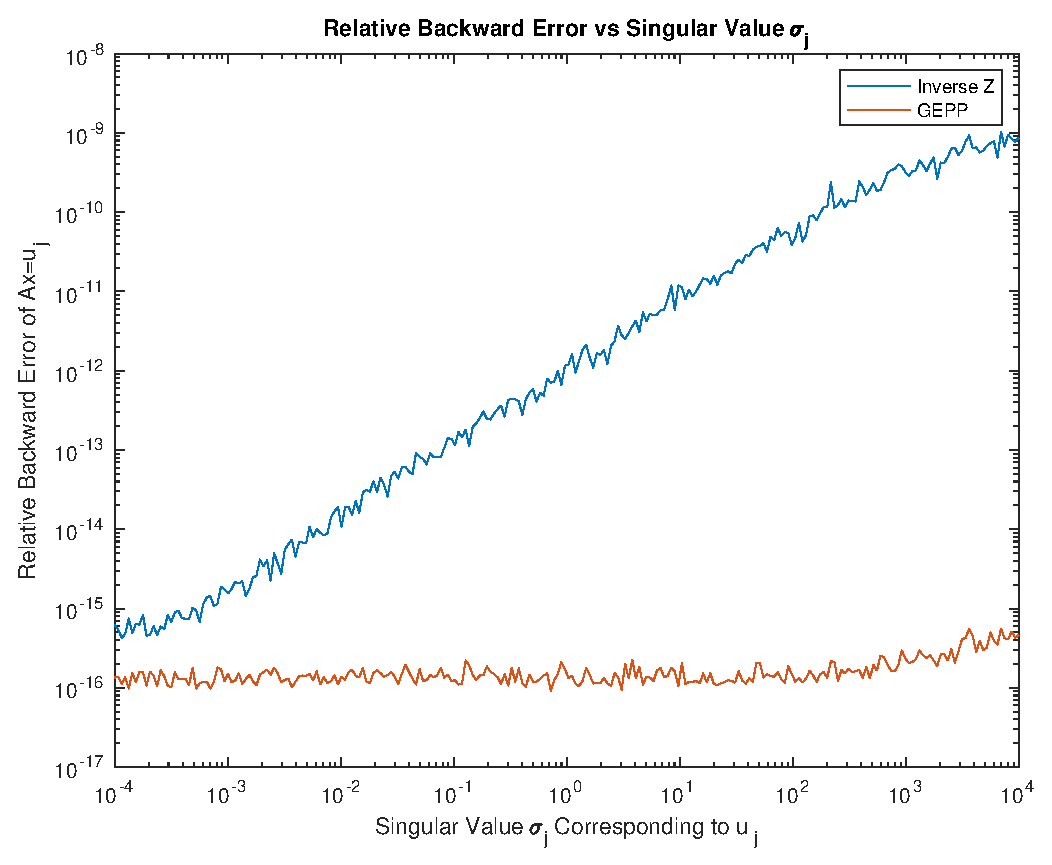
\includegraphics [width=4in]{Lab3_01.eps}

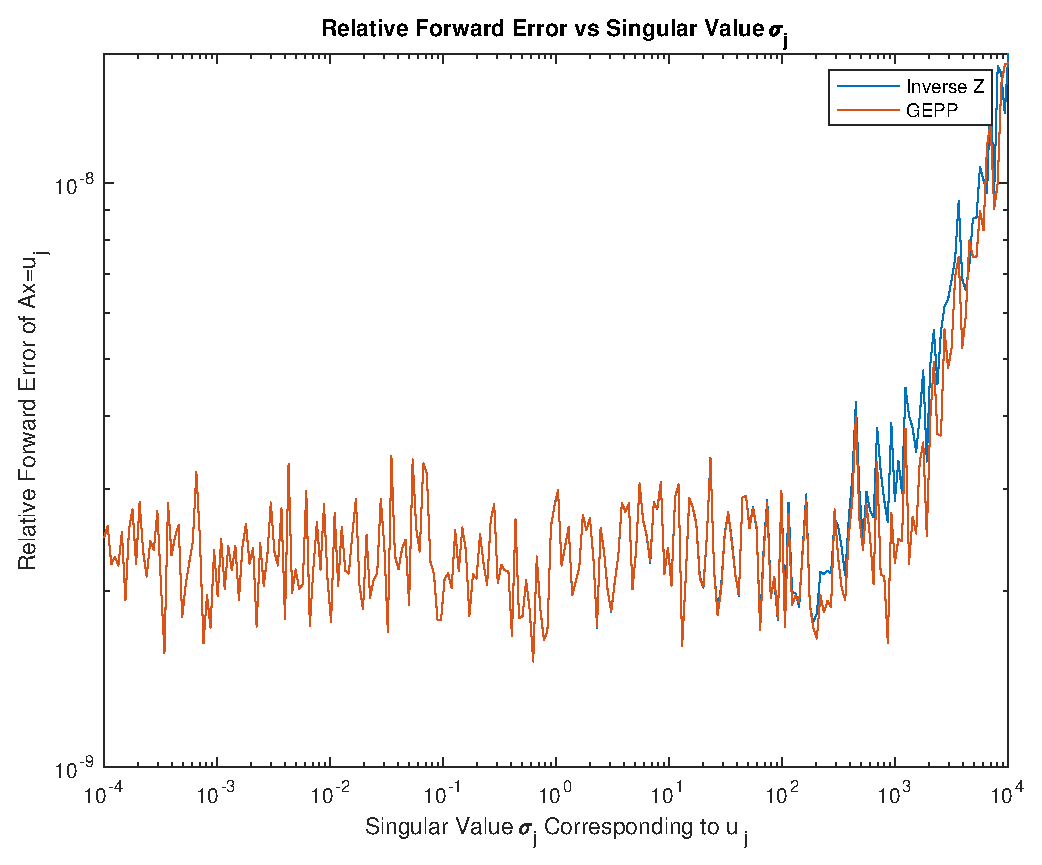
\includegraphics [width=4in]{Lab3_02.eps}
\begin{par}
From the first graph, we can see a major difference in relative backward error between using inverse Z and GEPP. Nearly 6 digits of accuracy were lost when the vector corresponding to the largest singular value was used. This is because the bound for relative backward error for inverse Z can be simplified to O(corresponding singular value / minimum singular value) as shown in problem \#5 in the attached PDF. This formula suggests that as the singular values corresponding to the left singular vectors used for b increase, the bound on relative backward error will also increase. This is reflected in the graph as the relative errors follow a pretty linearly increasing line as the corresponding singular value increases.
\end{par} \vspace{1em}
\begin{par}
To check the accuracy of this bound, I will calculate the ratio of the largest and smallest singular value, then multiplied by machine epsilon. Comparing this to the actual largest backward error from inverse Z will show that this bound is accurate.
\end{par} \vspace{1em}
\begin{verbatim}
fprintf('Bound = %e\n', (sigma_1 ./ sigma_n) .* eps());
fprintf('Largest actual error = %e\n', max(abs(rel_backward_err_inv2)));
\end{verbatim}

        \color{lightgray} \begin{verbatim}Bound = 2.220446e-08
Largest actual error = 1.023715e-09
\end{verbatim} \color{black}
    \begin{par}
Also from the first graph, the relative backward error of GEPP is around machine epsilon as predicted by the bound of O(machine epsilon). Therefore this error bound for GEPP is accurate.
\end{par} \vspace{1em}
\begin{par}
Lastly, the second graph showcasing relative forward error doesn't have a significant difference between the error from using inverse Z and using GEPP. The errors are generally of one magnitude of 10 or less, meaning that at most one digit of accuracy was lost when solving using inverse Z as compared to GEPP. From the condition number of A calculated below, we can approximate the bound to be around 10\^{}8 * 2 * 10\^{}-16 = 2 * 10\^{}-8. Hence, the error bound for forward error is also accurate.
\end{par} \vspace{1em}
\begin{verbatim}
fprintf('Condition number of A: %e\n', cond(A2));
fprintf('Largest actual error of inverse Z = %e\n', max(abs(rel_forward_err_inv2)));
fprintf('Largest actual error of GEPP = %e\n', max(abs(rel_forward_err_gepp2)));
\end{verbatim}

        \color{lightgray} \begin{verbatim}Condition number of A: 1.000000e+08
Largest actual error of inverse Z = 1.667858e-08
Largest actual error of GEPP = 1.604928e-08
\end{verbatim} \color{black}
    


\end{document}

